\begin{figure}[!htbp]
\centering
\textbf{(a) Largest trajectory gain}\par\smallskip
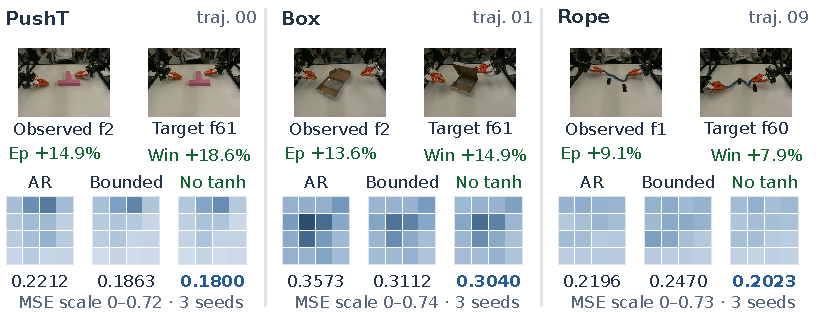
\includegraphics[width=\linewidth]{generated/qualitative_closest_v1/iws_largest.pdf}\par\medskip
\textbf{(b) Middle-ranked trajectory gain (fifth of ten)}\par\smallskip
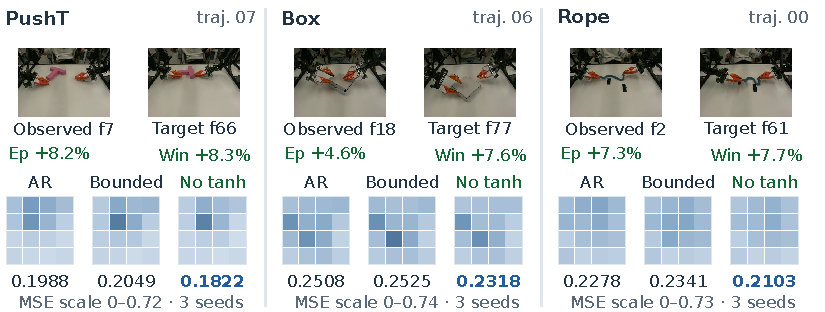
\includegraphics[width=\linewidth]{generated/qualitative_closest_v1/iws_median.pdf}\par\medskip
\textbf{(c) Smallest trajectory gain}\par\smallskip
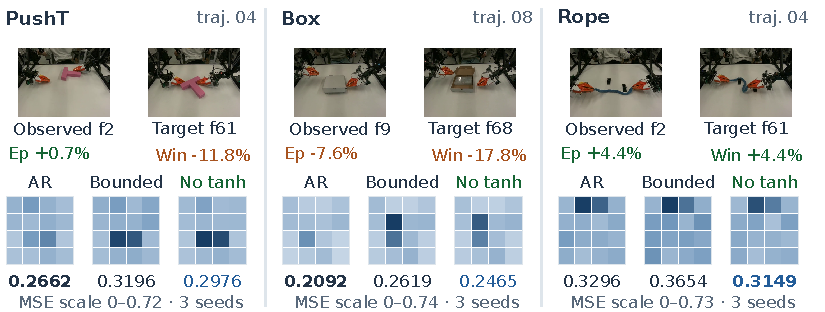
\includegraphics[width=\linewidth]{generated/qualitative_closest_v1/iws_smallest.pdf}
\caption{\textbf{Reserved manipulation recordings: gains and counterexamples.}
Posthoc trajectory ranks use no-$\tanh$ versus fixed AR; all panels show the
smallest registered start in that trajectory. Bounded and no-$\tanh$ are ShiftWM
and its ablation, respectively. Actual runner-up is bounded on PushT and AR
on Box/Rope. Recorded frames identify the identical observed input and withheld
target; grids show three-seed standardized feature MSE at offset 59 ($H=60$).
Bold scores are the lowest displayed point estimates within each case.
Each task uses one linear scale across all three methods and all three ranked
cases, with its limits printed below. Gains are relative MSE reductions, not
success-rate points. Trajectory and displayed-window gains can differ in sign.
Excerpts: RLA-WM/IWS; raw trajectories are not part of the public figure pack.}
\label{fig:closest-iws-gallery}
\end{figure}
